\documentclass[../main.tex]{subfiles}
\begin{document}

\subsection{Data}
Nine Solidity source files compiled with 4 solc versions (5, 6, 7, 8) times three optimization
settings (no optimization, runs = 1, runs = 999999).
Necessary changes where made to the source code to ensure compatibility with the different solc
version without altering the function of the contracts.
The runtime codes where segmented and the first segment skeletonized.

\subsection{Similarity}
Similarity for all code pairs was calculated via Jaccard Index on the bytebags of the contracts after filtering with the opcode filter:

\begin{lstlisting}[style=pymd]
(OP.is_log() or OP.is_storage() or OP.is_sys_op() or OP.is_env_info()
  or OP.is_block_info() or OP == opcodes.SHA3 or OP == opcodes.GAS)
\end{lstlisting}

\subsection{Clustering}
The clustering \figref{solc_bytebag_cluster} was done in Gephi (0.9.2) with the settings \figref{solc_bytebag_cluster_settings}.
Nodes with the same color have the same source code.
The graph is fully connected and the edge weights are determined by the similarity scores of the pairs.

\begin{figure*}[ht!]
  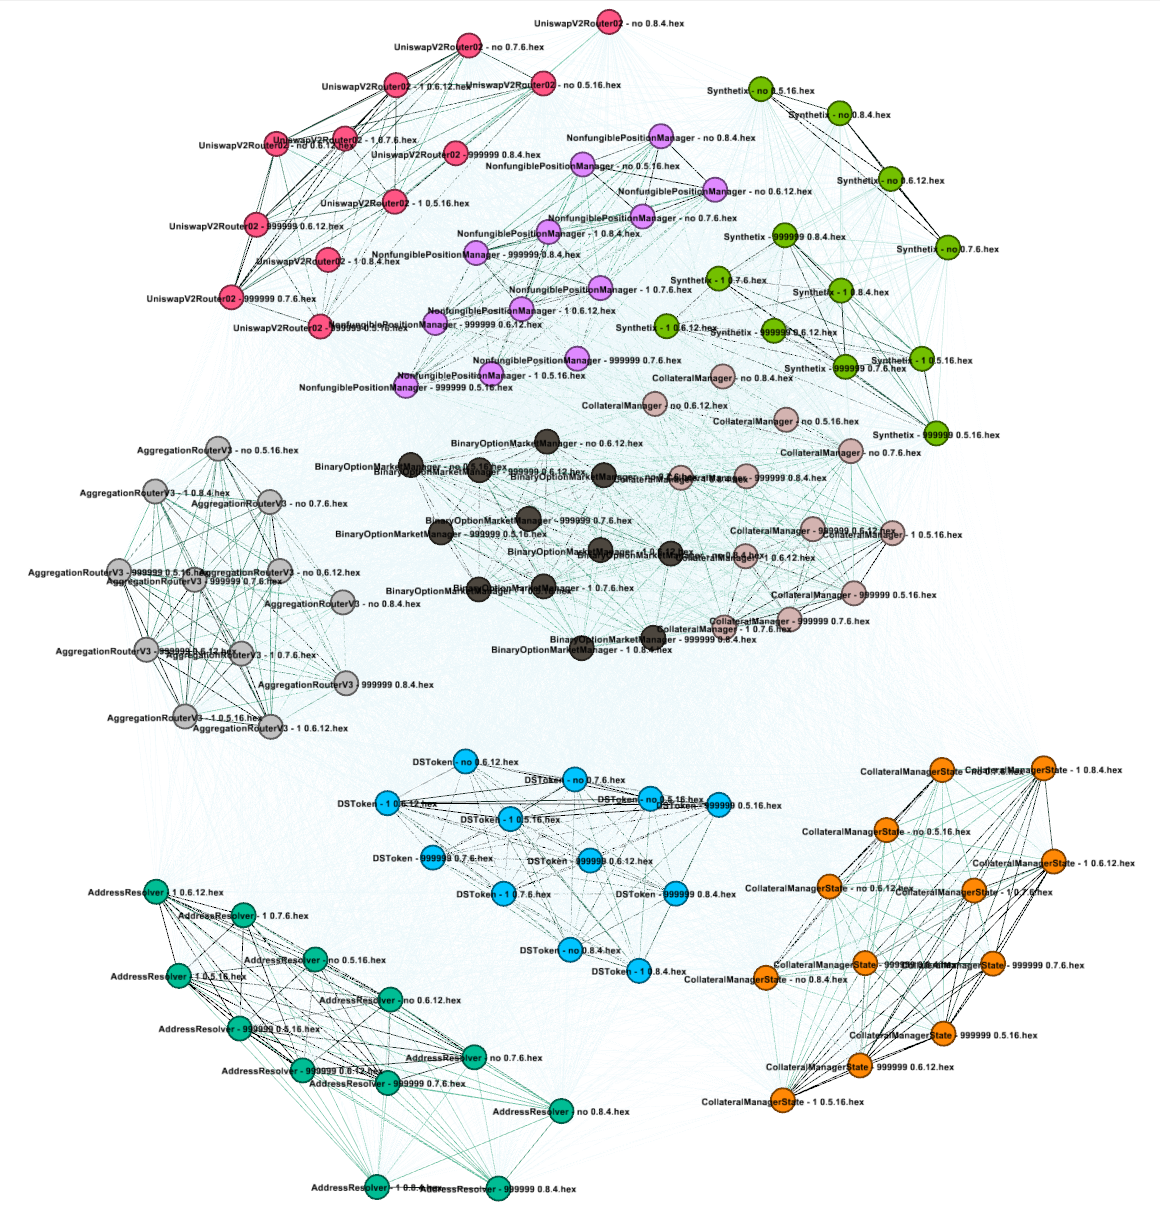
\includegraphics[width=\linewidth]{../../bsc-notes/clustering/clustering_result_many_solc_versions_byteBag_significant_only_2021-06-06_163755.png}
  \caption{solc versions bytebag}
  \label{fig:solc_bytebag_cluster}
\end{figure*}

\begin{figure*}[ht!]
  \centering
  \includegraphics[width=10cm]{../../bsc-notes/clustering/clustering_settings_many_solc_versions_byteBag_significant_only_2021-06-06_163526.png}
  \caption{Gephi settings}
  \label{fig:solc_bytebag_cluster_settings}
\end{figure*}

\subsection{Observation}
The clustering algo formed cohesive clusters, mostly due to the fact that the dataset is small and the contracts differ significantly in size alone.
Nonetheless, noticeable is that the Synthetix codes without optimization from all 4 solc versions form a cluster separate from the other Synthetix code.

\subsection{Analysis}
When comparing the frequency of the opcodes in \code{Synthetix - no 0.8.4.hex} and\\
\code{Synthetix - 999999 0.8.4.hex} these 7 op-codes show the highest change \tblref{opt_diff}.

\begin{table}[ht!]
  \centering
  \csvreader[
    tabular=rrlrrr,
    table head= dec & hex & op-code & no 0.8.4 & 999999 0.8.4 & diff\\\hline,
    head to column names]{csv/opt_diff.csv}{}{%
      \csvcoli & \texttt{\csvcolii} & \csvcoliii & \csvcoliv & \csvcolv & \csvcolvi}
  \caption{optimization differences}
  \label{tbl:opt_diff}
\end{table}

\code{54 0x36 CALLDATASIZE} is the most consistent across solc versions and optimization settings.

\code{59 0x3B EXTCODESIZE} is also very consistent. [csv]

\code{90 0x5A GAS} has a high absolute difference between the Synthetix contracts but it has higher differences across contracts.

\subsection{Interpretation}
The \code{RETURN} opcode should be filtered out since optimization drastically reduces its prevalence.

Optimization options change the codes more than solc version changes.

\end{document}
